\input sys/inputs.tex

\begin{document}

\bigheading{Stop rasizmu}

% \info{task_name}{infile}{outfile}{points}{timelimit}{memlimit}
% leave this values, if you are not interested
\info{networks}{stdin}{stdout}{100}{300 ms}{1 GB}

V Absurdistane po dlhý čas vládol silný rasizmuz. Biely neznášali čiernych a čierny, tí pracovali.
Verte alebo nie, táto neznášanlivosť vyústila do takých rozmerov, že čierny nemohli chodiť do
bielych reštaurácií a biely na čierne záchody. Nehovoriac o ostatných aspektoch života, poprípade
ľúbostných vzťahoch.

Dokonca to zašlo tak ďaleko, že každá rasa mala vlastnú cestnú sieť. Obe cestné siete sa skadali z
križovatiek, ktoré si môžeme predstaviť ako body v rovine, a ulíc, ktoré boli vždy rovné úsečky
spájajúce dve križovatky. Platilo, že žiadne dve ulice sa nepretínali a jednotlivé siete boli súvislé,
takže sa dalo dostať medzi každými dvoma križovatkami rovnakej farby. Siete však boli od seba
separované a teda neexistovala križovatka, patriaca do oboch sietí.

Uvedomelí občania Absurdistanu však pochopili, aký hlúpi boli v minulosti a zrušili všetky zákazy
obmedzujúce niektorú rasu. Ako prejav najväčšej spolupráce sa rozhodli spojiť svoje dve cestné siete
pomocou jednej spoločnej ulice. Otázkou však je, ktoré dve križovatky majú spojiť, aby naďalej
platilo, že žiadne dve ulice sa nepretínajú.

\heading{Úloha}

Na vstupe dostanete popis dvoch súvislých grafov, ktoré nezdieľajú žiaden vrchol a ktorých hrany sú
nepretínajúce sa úsečky. Nájdite dve križovatky, každú v inej siete, ktorých spojenie úsečkou nevytvorí
kríženie s inou už existujúcou úsečou.

\heading{Vstup}

Na vstupe dostanete popis bielej siete nasledovaný popisom čiernej siete. Popis siete vyzerá
nasledovne. Na prvom riadku sú dve čísla $N$ ($2 \leq N \leq 200\,000$) a $M$ ($1 \leq M \leq
700\,000$) -- počet vrcholov a hrán grafu. Nasleduje $N$ riadkov popisujúce pozície bodov, pomocou
dvojice celých čísiel $x_i$ a $y_i$ ($-1\,000\,000 \leq x_i,y_i \leq 1\,000\,000$). Body sú
očíslované od $1$ po $N$ v poradí, v akom sa vyskytli na vstupe. Za nimi je $M$
riadkov s číslami $p_i$ a $q_i$ $(1 \leq p_i \neq q_i \leq N)$, ktoré zodpovedajú začiatočnému a
koncovému vrcholu hrany.

\bigskip
V $30\%$ vstupných dát bude platiť, že $N,M \leq 3\,000$.

\heading{Výstup}

Na výstup vypíšte dve čísla $u$ a $v$ oddelené medzerou. $u$ je vrchol v bielej sieti a $v$ je
vrchol v čiernej sieti. Má platiť, že úsečka spájajúca tieto dva vrcholy nepretína žiadnu inú
existujúcu úsečku. Ak existuje viacero možností, vypíšte ľubovoľnú z nich.

\heading{Príklad}

\sampleIN
5 6
0 3
1 1
6 0
5 3
9 8
1 2
1 3
4 3
3 5
2 3
4 4
6 4
4 4
4 2
2 3
1 2
4 2
2 3
3 4
\sampleOUT
5 1
\sampleCOMMENT
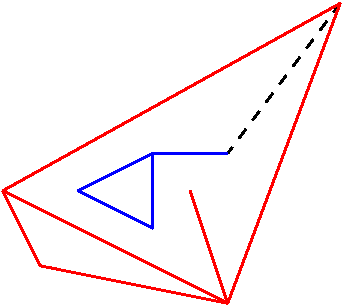
\includegraphics[height=4cm]{img/fig11.pdf}
\sampleEND

\end{document}
